% =====================================================================
%  tr03a —— 原文 pp.21–22
%  内容：§3.2 后半（Prym 簇的 2 阶元素、带符号差的实形式）、§3.3 起始
%  编号：式 (3.8)、式 (3.9)；定理 3.10
%  边界：起点 p.21 首段 "Hence, there is a short exact sequence …"（上块 tr-02
%        结束于 p.20 末的行间公式，不重复）；p.22 末句跨页至 p.23 首行
%        "…restrict ourselves here to / the simpler definition…"，按
%        STYLE_GUIDE §9「开始者写完」在本片段内写完，p.23 其后内容由 tr03b 接。
% =====================================================================

% [原文 p.21]

因此，存在短正合列 $0\to\pi_1(\Prym(S,\Sigma))\to\wedge\to 0$，由此 $\wedge\cong\pi_1(\Prym(S,\Sigma))$。所以 $\pi_1(\Prym(S,\Sigma))$ 是阿贝尔群，即
\[
\pi_1(\Prym(S,\Sigma))\cong H_1(\Prym(S,\Sigma),\Z).
\]

我们用 $\mathrm{P}[2]$ 表示 $\Prym(S,\Sigma)$ 中阶为 2 的元素，它们是 $V$ 中满足 $2x\in\wedge$ 的点 $x$ 的等价类。于是 $\mathrm{P}[2]$ 由 $\frac{1}{2}\wedge$ 模 $\wedge$ 给出；又因 $\wedge$ 无挠，有
\[
\mathrm{P}[2]\cong\wedge/2\wedge\cong H_1(\Prym(S,\Sigma),\Z_2).
\]

此外，$H^1(\Prym(S,\Sigma),\Z_2)\cong\Hom(H_1(\Prym(S,\Sigma),\Z),\Z_2)$，因此
\[
H^1(\Prym(S,\Sigma),\Z_2)\cong\Hom(\wedge,\Z_2)\cong\wedge/2\wedge\cong\mathrm{P}[2].
\]

由此，覆盖空间 $\mathrm{P}[2]$ 由 $\pi_1(\cA_{\mathrm{reg}})$ 在纤维的第一上同调（系数取 $\Z_2$）上的作用所决定。这一作用在 $n=2$ 的情形下见 [88]，在 $n>2$ 的情形下见 [12,16]。

% [Tutor Note: p.21 原文以 $\wedge$（楔积符号）记 Prym 簇 $V/\wedge$ 的晶格，p.20 已出现 "the quotient of a complex vector space $V$ by some lattice $\wedge$"；由 "$\wedge$ is torsion free" 与 $\wedge/2\wedge$ 是自由阿贝尔群的模 2 商可判断此处应为大写 $\Lambda$。原文全篇如此排印，译文照原样，不改。]

\para{带符号差的实形式} $\SU(p,p+q)$-Higgs 丛所在的轨迹由 $\SL(2p+q,\C)$-Higgs 丛上的对合 $\Theta_{\SU(p,p+q)}:(E,\Phi)\mapsto(E,-\Phi)$ 所固定；这些丛 $E$ 具有一个与 $\mathrm{I}_{p,p+q}$ 共轭的自同构，它将 $\Phi$ 映为 $-\Phi$，且其 $\pm1$ 特征空间的维数分别为 $p$ 与 $p+q$（另见例 2.14）。对合 $-\sigma$ 在偶次多项式上平凡地作用。此时，特征多项式由
\begin{equation}
\det(\eta-\Phi)=\eta^q(\eta^{2p}+a_2\eta^{2p-2}+\cdots+a_{2p-2}\eta^2+a_{2p}), \tag{3.8}
\end{equation}
给出，它定义谱曲线 $\pi:S\to\Sigma$，即
\[
S=\{0=\eta^{2p}+a_2\eta^{2p-2}+\cdots+a_{2p-2}\eta^2+a_{2p}\}\subset\operatorname{Tot}(K),
\]
其中 $\eta$ 是 $\pi^*K$ 的 重言截面（tautological section），$a_i\in H^0(\Sigma,K^i)$。

% [Tutor Note: p.21 "对合 $-\sigma$ 在偶次多项式上平凡地作用"的含义：在对合 $(E,\Phi)\mapsto(E,-\Phi)$ 下，特征多项式的 $k$ 次项系数 $a_k$ 变为 $(-1)^k a_k$，故偶次系数不变、奇次系数变号；在不动点（即 $\SU(p,p+q)$-Higgs 丛）上必有 $a_k=0$（$k$ 为奇数），于是 (3.8) 括号内只剩 $\eta$ 的偶次幂，谱曲线因而带有对合 $\sigma:\eta\mapsto-\eta$，其商给出 $p$ 重覆盖 $\bar\rho:\bar S\to\Sigma$。]

% [Tutor Note: p.21 记号混用：本页先写 "(3.8) … defines a spectral curve $\pi:S\to\Sigma$"，末尾又写 "We let $\pi:S\to\bar S$ be the double cover"；对照 p.21 末图（$\pi$ 标在 $S\to\bar S$ 上、$\rho$ 标在 $S\to\Sigma$ 上）以及 p.22 的 $K_S\cong\rho^*K^{2p}$、$K_{\bar S}\cong\bar\rho^*K^{2p}\otimes\bar\rho^*K^{-1}$，可知 $S\to\Sigma$ 应记作 $\rho$。译文照原文，读者以图示与 p.22 为准。]

尽管当 $q\ne 0,1$ 时谱数据尚不清楚，但在 $q=0$ 的情形下，[89, Chapter 6] 与 [91] 通过考察 $\U(p,p)$-Higgs 丛 $(W_1\oplus W_2,\Phi)$ 给出了描述：当满足 $\Lambda^pW_1\cong\Lambda^qW_2^*$ 时，它们对应于 $\SU(p,p)$-Higgs 丛（$q=1$ 的情形在 [82] 中通过 cameral 数据研究）。此外，当 $q=0$ 时，曲线 $S$ 是黎曼面 $\Sigma$ 的 $2p$ 重覆盖，在 $a_{2p}$ 的 $4p(g-1)$ 个零点处分歧，并带有自然对合
\begin{equation}
\sigma:\eta\mapsto-\eta \tag{3.9}
\end{equation}
其不动点恰为该覆盖的分歧点。

% [Tutor Note: p.21 原文 "$\Lambda^pW_1\cong\Lambda^qW_2^*$" 右端指数应为 $p$：此处讨论的是 $q=0$ 的 $\SU(p,p)\subset\SL(2p,\C)$ 情形，条件 $\det(W_1\oplus W_2)\cong\cO$ 给出 $\Lambda^pW_1\cong\Lambda^pW_2^*$。500 dpi 裁图复核原文确印作 $\Lambda^q$，译文照原文。]

$S$ 在 $\sigma$ 作用下的商定义了 $K^2$ 全空间中的 $p$ 重覆盖 $\bar\rho:\bar S\to\Sigma$，其方程由 $\xi^p+a_1\xi^{p-1}+\cdots+a_{p-1}\xi+a_p=0$ 给出，其中 $\xi=\eta^2$ 是 $\bar\rho^*K^2$ 的 重言截面。由于 $\bar S$ 是光滑曲线的商，它也是光滑的。我们令 $\pi:S\to\bar S$ 为由上述商给出的二重覆盖：
\begin{center}
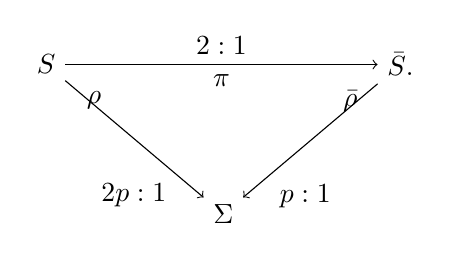
\begin{tikzpicture}[x=1cm, y=1cm]
  \node (S) at (0,1.35) {$S$};
  \node (Sb) at (4.5,1.35) {$\bar{S}$.};
  \node (Sig) at (2.25,-0.55) {$\Sigma$};
  \draw[->] (S) -- node[above] {$2:1$} node[below] {$\pi$} (Sb);
  \draw[->] (S) -- node[pos=0.33,above left] {$\rho$} node[pos=0.80,below left] {$2p:1$} (Sig);
  \draw[->] (Sb) -- node[pos=0.33,above right] {$\bar\rho$} node[pos=0.80,below right] {$p:1$} (Sig);
\end{tikzpicture}
\end{center}

% [原文 p.22]

我们分别用 $g_S$ 与 $g_{\bar S}$ 表示 $S$ 与 $\bar S$ 的亏格。由于余切丛的典范丛平凡，而 $K^2$ 的典范丛为 $\bar\rho^*K^{-1}$，由伴随公式（adjunction formula）可得 $K_S\cong\rho^*K^{2p}$ 与 $K_{\bar S}\cong\bar\rho^*K^{2p}\otimes\bar\rho^*K^{-1}$。于是
\[
g_S=4p^2(g-1)+1,
\]
\[
g_{\bar S}=(2p^2-p)(g-1)+1.
\]

% [Tutor Note: p.22 的 $g_S$、$g_{\bar S}$ 可用两步 Riemann--Hurwitz 验算：$\bar S\to\Sigma$ 为 $p$ 重覆盖，判别式 $\operatorname{disc}(\xi^p+a_1\xi^{p-1}+\cdots+a_p)$ 是 $K^{2p(p-1)}$ 的截面、零点数为 $4p(p-1)(g-1)$，故 $2g_{\bar S}-2=p(2g-2)+4p(p-1)(g-1)$，即 $g_{\bar S}=(2p^2-p)(g-1)+1$；再由 $S\to\bar S$ 为 $2:1$、分歧于 $a_p$（即 (3.8) 中的 $a_{2p}$）的 $4p(g-1)$ 个零点，得 $2g_S-2=2(2g_{\bar S}-2)+4p(g-1)=8p^2(g-1)$，即 $g_S=4p^2(g-1)+1$。两式自洽。]

$\SU(p,p)$-Higgs 丛的谱数据于是可由如下描述的 $\U(p,p)$-Higgs 丛的谱数据推出：

\begin{thm}{3.10（[91]）}
给定一个具有非奇异谱曲线的 $\U(p,p)$-Higgs 丛，可以构造一个对 $(S,M)$，其中
\begin{enumerate}[label=(\alph*),leftmargin=2.2em]
\item 曲线 $\rho:S\to\Sigma$ 是 $\Sigma$ 的一条不可约非奇异 $2p$ 重覆盖，在 $K$ 的全空间中由方程 $\eta^{2p}+a_1\eta^{2p-2}+\cdots+a_{p-1}\eta^2+a_p=0$ 给出，其中 $a_i\in H^0(\Sigma,K^{2i})$，而 $\eta$ 是 $\rho^*K$ 的 重言截面。曲线 $S$ 带有一个对合 $\sigma$，其作用为 $\sigma(\eta)=-\eta$；
\item $M$ 是 $S$ 上的一个线丛，使得 $\sigma^*M\cong M$。
\end{enumerate}
反之，给定满足 (a) 与 (b) 的对 $(S,M)$，存在一个相伴的稳定 $\U(p,p)$-Higgs 丛，其谱曲线如 (a) 所述。
\end{thm}

% [Tutor Note: p.22 定理 3.10 中的系数 $a_1,\dots,a_p$ 与 (3.8) 中的 $a_2,a_4,\dots,a_{2p}$ 是同一组系数：定理给出 $a_i\in H^0(\Sigma,K^{2i})$，而 (3.8) 给出 $a_i\in H^0(\Sigma,K^i)$，故 $a_i^{(3.10)}=a_{2i}^{(3.8)}$；把定理的方程与 (3.8) 括号内的部分逐项对照即可验证（$i=1,\dots,p$ 对应 $2i=2,\dots,2p$）。]

从 (3.8) 中所描述的 $\SU(p,p+q)$-Higgs 丛的特征多项式的结构可以看出：当 $q\ge 1$ 时，一般地（generically），该多项式定义一条可约曲线，因此所有 $\SU(p,p+q)$-Higgs 丛都位于 Hitchin 纤维化的判别式轨迹上方的纤维中。大多数其他非分裂实形式所给出的 Higgs 丛也位于 Hitchin 纤维化的非正则轨迹上方，如 [89] 所示。

更一般地，人们会问：给定的 Higgs 丛集合是否总能表示为 Hitchin 纤维化正则轨迹上方的元素？对秩 2 Higgs 丛的情形，Wentworth 与 Wolf 在 [102] 中证明：对曲面群到 $\SL(2,\C)$ 的每个非初等表示，都存在一个黎曼面结构，使得与该表示相伴的 Higgs 丛位于 Hitchin 纤维化的判别式轨迹之外。当 $n\ge 3$ 时，以及对任何其他群，该问题仍然未决：事实上，由 [102, Remark 3.iv.] 可知，在他们定理的任何推广中都会出现障碍，而其中一些障碍来自 $\SL(n,\C)$ 的其他实形式，后者总是位于判别式轨迹中。特别地，他们的工作涉及 Gallo-Kapovich-Marden 的一个结果，而该结果尚需推广到更高秩。

\subsection{Hitchin 纤维化的奇异轨迹}

在本讲义各处我们都说过：Hitchin 底中的点 $\omega\in\cA_{G_{\C}}$ 是正则的，当它所定义的谱曲线 $S$ 是光滑的--等价地，我们说过它是奇异的，当由 Higgs 场的特征多项式 (3.5) 所定义的相应谱曲线是奇异的。然而，对 Hitchin 底作分层还有更为精细、也更有用的方式，例如 [79] 中所使用的那些（关于这些分层的进一步描述见 [30]）。不过，我们在此只限于采用奇异点较为简单的定义，
% [原文 p.23]
并就由此产生的某些几何与若干未决问题略作评论。

% [Tutor Note: p.22 §3.3 首句 "the spectra curve" 应为 "spectral curve"（下一句即改回 spectral）；p.22 末行 "…outside the discriminant locus of the Hitchin fibration For $n\ge 3$…" 在 fibration 与 For 之间脱一句号，译文按两句话处理。]
